\subsection{Usage and integration}
The produced system is able to interact seamlessly with existing Ruby code, via type annotation on collection objects.

\begin{lstlisting}[
  language=Ruby,
  label=lst:example_snippet,
  caption=Redirecting a computation through the RubiCL library via type annotation.
]
  # Sequential stdlib code
  (1..1_000_000)
    .map { |x| x + 15 }
    .select { |y| y % 15 == 0 }

  # Parallel code using RubiCL
  (1..1_000_000)[Int]
      .map { |x| x + 15 }
      .select { |y| y % 15 == 0 }[Fixnum]
\end{lstlisting}


When a user is sure that all objects within an \verb|Enumerable| are of a single, basic type, they can append a type declaration to the container. This declaration lies within the method pipeline and states the equivalent C type, the object is then wrapped by the RubiCL execution environment.

Further method calls are captured by the \verb|Device| instance handling the dataset, and pushed onto a work-queue.

Eventually, a result is requested, either by a user casting back to a Ruby object class, or by performing a terminal action such as summation. The work-queue is then optimised and mapped to OpenCL kernels, dispatched to the target compute device.

The produced wrapper solution for including additional functionality to the Ruby runtime is ideal. Programmers must only grasp the concept of annotating type-conversion at the beginning and end of any calculation pipelines. All other syntax of the library is identical to normally-written Ruby code.

Despite the simplicity of the library's presented interface, there is a lot of work going on behind the scenes. The technical details of which will be discussed in the \emph{Implementation} chapter.

As an overview, the steps undertaken by the RubiCL library for the example given in Figure~\ref{lst:example_snippet} include:
\begin{itemize}
  \item Moving the dataset elements into continuous memory addressable by the compute device.
  \item Recording the loaded dataset type, to allow static type-system operations.
  \item Parsing the \verb|block| argument of the \verb|#map| task's bytecode and constructing an equivalent C99 expression.
  \item Parsing the \verb|block| argument of the \verb|#select| task's bytecode and constructing an equivalent C99 expression.
  \item Inserting a \verb|Map| task at the beginning of the \verb|TaskQueue| to convert from Ruby objects to C \verb|int|s.
  \item Inserting a \verb|Map| task at the end of the \verb|TaskQueue| to convert from C \verb|int|s back to Ruby objects.
  \item Simplifying the $4$ tasks in the \verb|TaskQueue| to a single, \verb|MapFilter| task via \emph{fusion}.
  \item Generating the OpenCL kernel required to perform the \verb|MapFilter| task.
  \item Executing the produced kernel on the compute device, recording metrics.
  \item Returning the resultant values as a Ruby array.
\end{itemize}

\subsection{Software architecture}
The library is constructed from the following set of modules and classes, alongside their responsibilities:
\begin{description}
  \item[RubiCL] Environment singleton and top level namespace.
\end{description}


Figure~\ref{fig:rubicl_components} shows the interactions between classes during a typical parallelised computation.
\begin{sidewaysfigure}[h]
  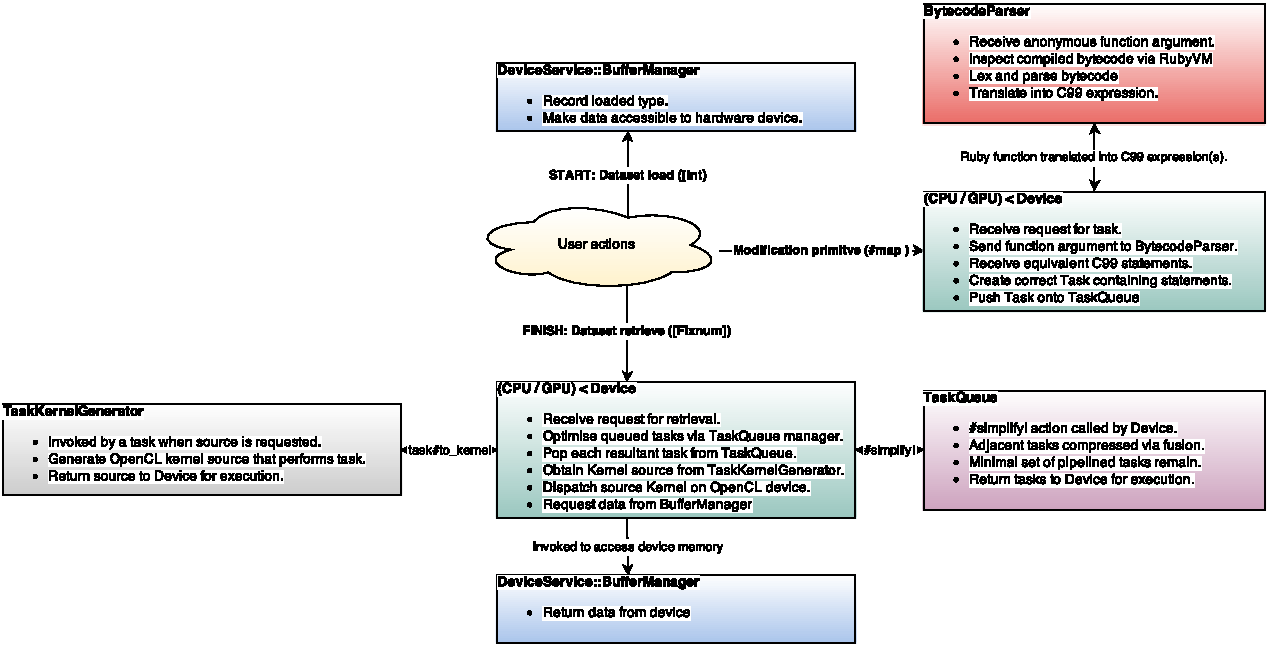
\includegraphics[width=\textwidth]{./figures/arch_components.pdf}
  \caption{An overview of the interacting software components during the lifetime of a typical computation}
  \label{fig:rubicl_components}
\end{sidewaysfigure}

\subsection{Interacting with hardware devices}
Interaction with hardware devices present on the system occurs via native extensions. These extension modules are mixed-into device singletons, created when the library is first launched. Figure~\ref{fig:rubicl_devices} shows the functionality of these singletons and their subcomponents.

\begin{figure}[h]
  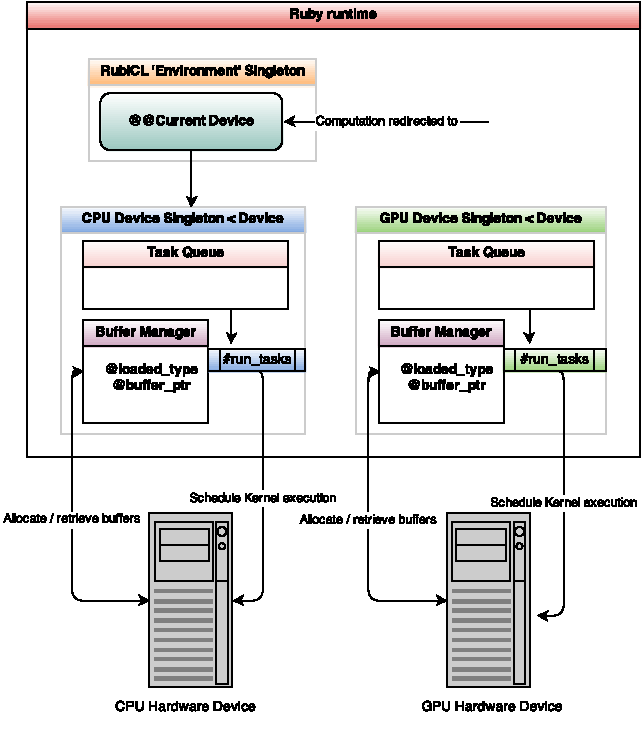
\includegraphics[width=0.8\textwidth]{./figures/arch_diagram.pdf}
  \caption{The RubiCL runtime maintains singletons for each device, used to trigger management functions and execute kernels.}
  \label{fig:rubicl_devices}
\end{figure}

Both \verb|CPU| and \verb|GPU| objects, tasked with managing device state, inherit from a common \verb|Device| superclass. The main difference in their implementation is differing initialisation procedure. Having two device types allows target-specific optimisation by the code generator, shown later.

The \verb|Device| subclasses delegate maintaining the list of tasks to a \verb|TaskQueue| object. In addition, they lack the ability to call memory management functions on devices and instead trigger functionality via an instance of \verb|DeviceService::BufferManager|.

Implementing all device logic that does not require hardware interoperability in Ruby made the system much easier to test. The time taken for the device control flow to execute is insignificant compared to the time taken for data processing. Writing this section in C would have been misguided as the performance benefits would not be worth the impaired rate of development.
